% !TeX root = ../thuthesis-example.tex

\chapter{相关研究综述}
本章主要介绍了时间序列对称模式挖掘涉及的
基本概念和国内外相关研究。
其中2.1节定义了时间序列和对称模式,
并对全局和分段对称模式挖掘进行了形式化定义;
2.2节介绍了基于序列形状和数学模型的时间序列相似性度量方法;
2.3节分析了基于相似性检索和时序分解的时间序列模式挖掘方法。
研究发现,当前时间序列分析领域并不存在有关对称模式挖掘的成熟方法。

\section{时间序列与对称模式}
大数据和物联网的发展与融合产生了大量的工业数据,
本文主要研究其中的时间序列数据。
接下来,本节将对时间序列、时间子序列、
对称子序列以及对称模式等进行定义。
\cite{DBLP:journals/ijsi/GaoSW21}。

\begin{definition}
  时间序列是由数据和其对应时间戳按顺序排列而成的一组数列\cite{DBLP:journals/csur/EslingA12}。

  具体而言,在一条数据序列$X = \left( p_1,p_2,\dots,p_n \right)$中,
  $p_i$指第$i$个数据点,每个数据点$p_i$都由一个时间戳$t_i$和值$x_i$
  组成,因此,$p_i$又可以表示成$\left( t_i,x_i \right)$。
\end{definition}

\begin{definition}
  反转时间序列指对原始时间序列的所有数据点前后逆序排列后得到的时间序列。

  参考转置矩阵的定义\cite{DBLP:conf/vecpar/HishinumaHT16},
  本文提出了反转时间序列。具体而言,如果原始时间序列
  为$X = \left( p_1,p_2,\dots,p_n \right)$,那么,其反转时间序列为
  $X = \left( p_n,p_{n-1},\dots,p_1 \right)$。
\end{definition}

\begin{definition}
  时间子序列指时间序列中点的顺序子段。

  从时间序列$X=\left( p_1,p_2,\dots,p_n \right)$中随机从第$i$个点开始
  截取一段连续的子序列$S = \left( p_i,p_{i+1},\dots,p_{i+m-1} \right)$,
  则$S$称为$X$的时间子序列。 
\end{definition}

\begin{definition}
  对称时间序列指经过某种变换,前后状态等价或相同的时间序列
  \cite{DBLP:journals/pami/NackmanP85}。

  换言之,如果时间序列$S$沿某个对称中心截断后,
  中心两侧的序列能够互为镜像,那么,$S$则为对称时间序列。
  如果$S$同时是$X$的时间子序列,则称$S$为$X$的对称时间子序列。
\end{definition}

\begin{definition}
  对称模式包含两种类别,全局对称模式和分段对称模式。

  全局对称模式指具有全局对称性的时间序列,
  而分段对称模式指从具有分段对称性的时间序列挖掘出的数量
  最多且不重叠的对称子序列组成的集合\cite{2022968}。 
  
\end{definition}

综合以上定义,挖掘全局对称模式的算法可以形式化定义为,
给定一个时间序列$X$和由专家指定或自适应生成的全局对称度阈值$d$,
满足公式~\ref{eq:global_symmetric_pattern}的时间序列即属于
全局对称模式$M$。
\begin{equation}
  M = \{X | symmetry(X) \leq d\}
  \label{eq:global_symmetric_pattern}
\end{equation}
而挖掘分段对称模式的算法可以形式化定义为,给定一个时间序列$X$和
子序列长度约束$w$,通过确定子序列对称度阈值$d$,
计算时间序列$X$中长度为$w$且对称度小于阈值$d$的
所有不重叠时间子序列$S$组成的分段对称模式集合$M$,
同时保证时间子序列的数目最多,
优化目标和约束如式~\ref{eq:symmetric_pattern}所示

\begin{equation}
  \begin{split}
    & \max \left| M \right| \\
    & s.t. symmetry \left( S \right) \leq d, \qquad 1 \leq i \leq \left| M \right|,S \in M \\
    & \left| S \right| = w, \qquad \qquad \qquad \quad 1 \leq i \leq \left| M \right|,S \in M \\
    & S \cap T = \emptyset, \qquad \qquad \qquad S,T \in M,S \neq T
  \end{split}
  \label{eq:symmetric_pattern}
\end{equation}

图~\ref{fig:symmetric_result}展示了全局和分段对称模式挖掘的结果,
计算得到的对称模式可以为后续的数据分析和序列预测提供关键参考。
\begin{figure}
  \centering
  \subcaptionbox{全局对称模式\label{fig:global_symmetry_result}}
    {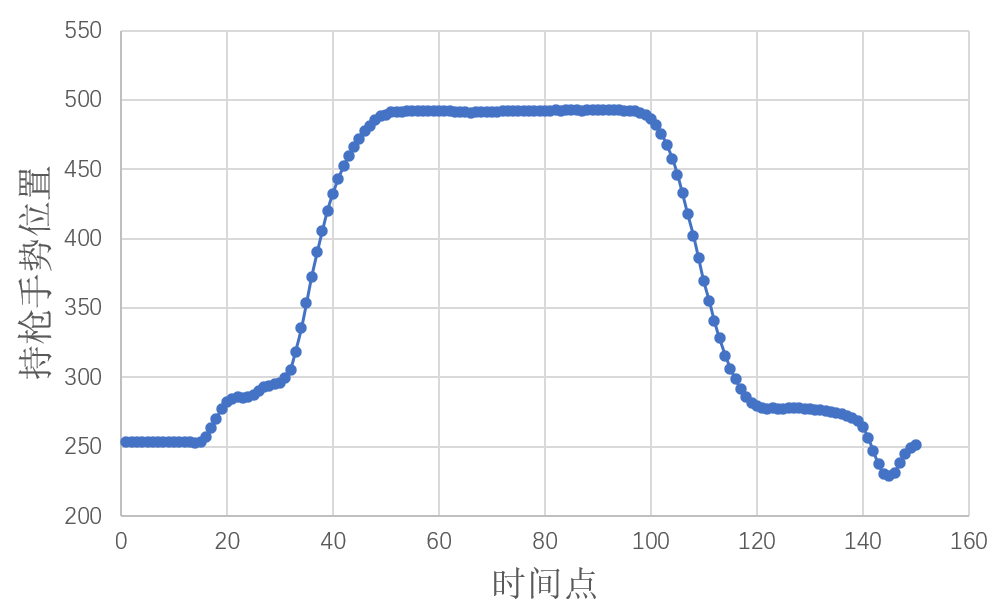
\includegraphics[width=0.49\linewidth]{global_symmetry_result.png}}
  \subcaptionbox{分段对称模式\label{fig:segmented_symmetry_result}}
    {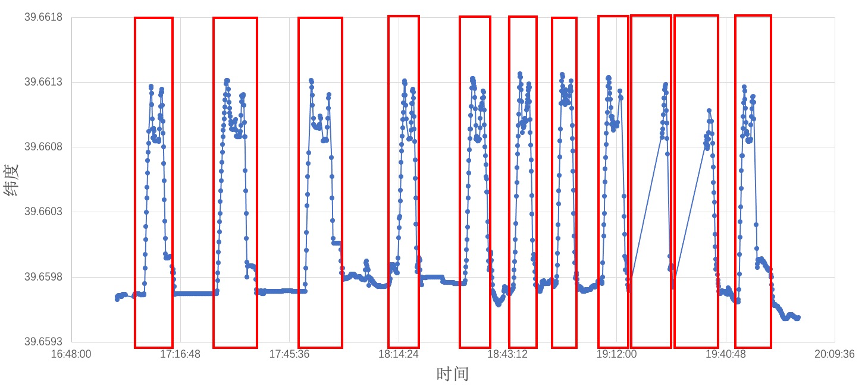
\includegraphics[width=0.49\linewidth]{symmetric_result.png}}
  \caption{对称模式挖掘结果}
  \label{fig:symmetric_result}
\end{figure}

\section{时间序列相似性度量}
时间序列对称性的度量,本质上就是时间序列两段子序列的相似性度量。
因此,相似性度量算法的选择与研究对于时间序列对称模式挖掘意义重大。
现有的时间序列相似性度量方法大体可以划分为两种,
一种是基于序列形状的相似性度量方法,
另一种是基于数学模型的相似性度量方法
\cite{DBLP:journals/vldb/SuLZZZ20}。
下面将详细介绍这两种方法的国内外研究现状。

\subsection{基于序列形状的相似性度量方法}
在序列相似性度量问题中,欧氏距离是一种最为常见的
基于距离和形状的方法。
例如,Yeh等人提出的Matrix Profile方法便是
利用欧氏距离度量子序列的相似性
\cite{DBLP:conf/icdm/YehZUBDDSMK16}。
对于长度相同的时间序列,通过计算每两点之间的距离然后累积求和,
距离越小则相似度越高。这种方法的直观表达可以
用式~\ref{eq:euclidean_distance}来表示。
假如$S=\left(\left(t_1,x_1 \right),\left(t_2,x_2\right),\dots,\left(t_n,x_n\right)\right)$
和$Q=\left(\left(t_1,y_1 \right),\left(t_2,y_2\right),\dots,\left(t_n,y_n\right)\right)$是两条时间序列,则这两条时间序列基于欧氏距离的相似度则可以用式~\ref{eq:euclidean_distance}来计算
\begin{equation}
  D\left(S,Q\right) = \sqrt{\sum_{i=1}^{n}{\left| x_{i}-y_{i} \right|^{2}}}
  \label{eq:euclidean_distance}
\end{equation}

基于欧氏距离的相似性度量方法不仅计算简单、易于理解,
计算效率也较高,
当时间序列数据点为多个维度时同样适用。然而,
欧氏距离要求匹配的两个
时间序列的长度相同,并且由于是一一对应的同步匹配算法,
当出现数据缺失和平移等状况时,会导致欧氏距离的度量结果
存在很大误差
\cite{DBLP:journals/pvldb/DingTSWK08}。
例如两个序列$A=\left(2,2,5,5,15,15\right)$和
$B=\left(2,5,5,15,15,15\right)$的欧氏距离为109,
然而两个序列的相似度非常高,只是$A$相对于$B$在水平方向上
向右发生了平移。
相比于时间序列,字符串相似性的度量方法种类更多,研究更广。因此,
可以采用离散化和符号映射的方法将时间序列转化为字符串序列,
则时间序列相似性度量方法由连续数据的距离度量转换成了离散数据
的距离度量。基于此,Eamonn Keogh和Jessica Lin在2002年
发明了SAX算法\cite{DBLP:conf/dmkd/LinKLC03},
用于将时间序列转化为字符串。
图~\ref{fig:SAX}展示了将时间序列利用SAX符号化为字符串序列的流程,
首先将时间序列数据进行归一化处理,使之具有高斯分布的特征。
然后将新序列降维并用分段聚合近似(PAA)表示,根据将高斯序列划分
成任意数量等概率区间的断点序列B,对PAA处理之后的序列完成符号化。
将时间序列转换为字符串序列之后,
便可用字符串之间的距离表示时间序列的相似性。
字符串距离度量算法相对多样,接下来将介绍3种经典的字符串距离度量算法。
\begin{figure}
  \centering
  \subcaptionbox{原始时间序列\label{fig:SAX-a}}
    {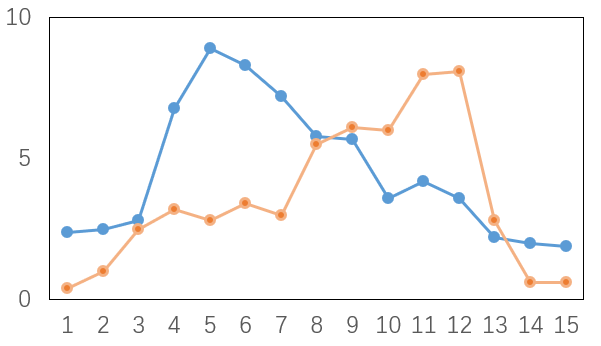
\includegraphics[width=0.43\linewidth]{SAX-a.png}}
  \subcaptionbox{高斯分布归一化处理\label{fig:SAX-b}}
    {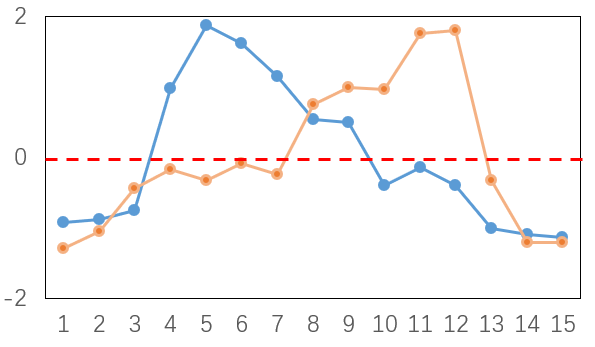
\includegraphics[width=0.43\linewidth]{SAX-b.png}}
  \subcaptionbox{分段聚合近似\label{fig:SAX-c}}
    {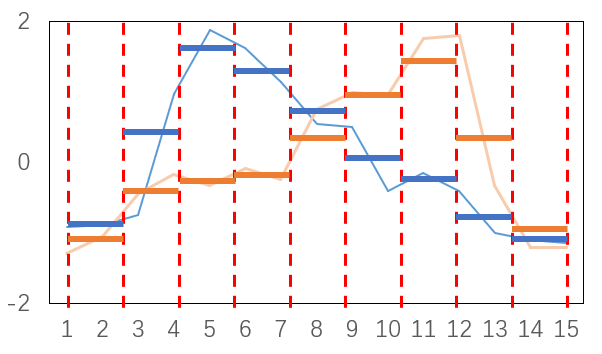
\includegraphics[width=0.43\linewidth]{SAX-c.png}}
  \subcaptionbox{利用断点列表符号化\label{fig:SAX-d}}
    {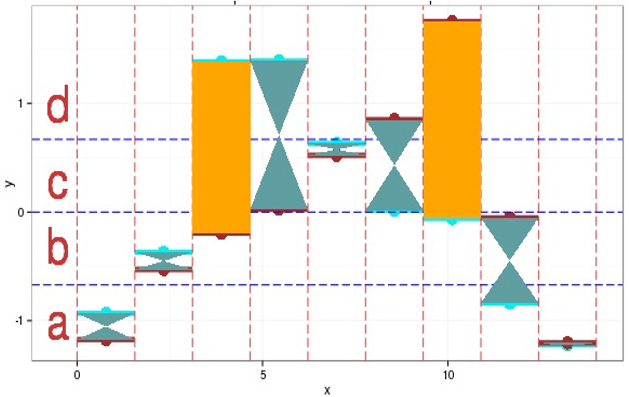
\includegraphics[width=0.43\linewidth]{SAX-d.png}}
  \caption{SAX符号化时间序列算法流程}
  \label{fig:SAX}
\end{figure}

编辑距离原本是对两个字符串差异程度的度量,
其测量方式是计算至少需要多少次编辑操作才能
将一个字符串转化为另一个,
编辑操作包括插入、删除和替换\cite{DBLP:journals/prl/Gorecki14}。
例如两个序列$A=\left(a,b,c,a,b\right)$和$B=\left(a,c,a,b,b\right)$的编辑距离为2。编辑距离可以通过动态规划的算法思想进行计算,
式~\ref{eq:edit_distance}展示了编辑距离的动态规划方程,
当$A$和$B$两个序列的尾字符不相同时,可以通过修改,插入或者删除$A$的
尾字符使其与$B$序列相同,从中选择最小值作为序列的编辑距离。


\begin{equation}
  DP(i, j)= \begin{cases}DP(i-1, j-1), & A_{i}=B_{j} \\
    \min \left\{\begin{array}{c}
    D P(i-1, j-1)+1 \\
    D P(i-1, j)+1 \\
    D P(i, j-1)+1
    \end{array}\right. , & A_{i} \neq B_{j}
  \end{cases}
  \label{eq:edit_distance}
\end{equation}

最长公共子序列(LCSS)也可以用来度量两个字符串序列的相似性,
如果一个序列$S$同时是字符串$A$和$B$的子序列
\cite{DBLP:conf/spire/BergrothHR00}。且是所有符合此条件
的最长序列,那么序列S的长度则可以表示两个序列的距离,
并用$S$的长度和$A$、$B$字符串长度最大值的比值衡量两个字符串的相似性。
LCSS也是一种非常经典的利用动态规划思想求解的字符串距离度量算法,
其计算公式如式~\ref{eq:LCSS}所示

\begin{equation}
  D P(i, j)= \begin{cases}0, & i=0 \text { or } j=0 \\ D P(i-1, j-1)+1, & i, j>0 \text { and } A_{i}=B_{j} \\ \max \begin{cases}D P(i-1, j) \\ D P(i, j-1)\end{cases} & i, j>0 \text { and } A_{i} \neq B_{j}\end{cases}
  \label{eq:LCSS}
\end{equation}

除了经典方法,还有一些较为新颖、正处在发展中的字符串距离度量方法,
例如,带惩罚的编辑距离(ERP)方法\cite{DBLP:conf/vldb/ChenN04}。
ERP算法也是一种基于编辑距离的
字符串距离度量算法。相比经典编辑距离,ERP算法是将匹配过程中插入或删除
时缺少值的一方视为一个gap算子。也就是说,当字符串序列$A$和$B$进行匹配时,
若要在$A_i$插入一个来自$B$序列的$B_j$使得$A$和$B$更为接近时,那么
在距离度量时将不再简单的增加一次编辑操作,而是将$B_j$与$gap$算子的距离视为
本次编辑操作的代价。式~\ref{eq:ERP}展示了ERP方法的计算公式,相比经典编辑距离,
ERP通过指定gap的方式使得距离度量更加灵活,不再是简单编辑操作的数量。
然而,ERP方法的效果和准确率极大地依赖gap的选取,不仅增加了模型的复杂度,
而且不适用于变化剧烈的序列。

\begin{equation}
  D P(i, j)= \begin{cases}\sum_{k=1}^{j}\left|B_{k}-g a p\right|, \qquad \qquad \qquad \qquad \quad i=0 \\
    \sum_{k=1}^{i}\left|A_{k}-g a p\right|,\qquad \qquad \qquad \qquad \quad j=0 \\
    \max \left\{\begin{array}{l}
    \left|A_{i}-B_{j}\right|+D P(i-1, j-1) \\
    \left|A_{i}-\operatorname{gap}\right|+D P(i-1, j) \\
    \left|B_{i}-\operatorname{gap}\right|+D P(i, j-1)
    \end{array}, \quad i, j>0 \text { and } A_{i} \neq B_{j}\right.\end{cases}
    \label{eq:ERP}
\end{equation}

尽管通过符号化的方法将时间序列转化为字符串之后可以通过字符串距离度量
时间序列的相似性,然而,在处理过程中由于降维、平滑和离散化等操作,
必然导致时间序列原始信息的缺失。况且,基于编辑距离的字符串匹配方式
从根本上来说属于部分匹配,通过编辑操作将不匹配的点删除,这种方式度量
出来的距离没有体现全局时间序列的特征。而ERP算法也只是将不匹配点与
一个固定点gap匹配,过于简单粗暴,在不匹配点差距较大时性能下降明显。
而动态时间扭曲算法(DTW)\cite{DBLP:conf/kdd/BerndtC94,DBLP:conf/sdm/KeoghP01}
则是一种直接计算两个时间序列之间相似性的全局
匹配算法。尽管具有相似性的两个时间序列在距离和形状上相近,但是,
由于时间序列的数据维度高,数据类型多样,任何两个序列都有可能存在随机
差异,包括平移伸缩、数据缺失和噪声等。因此,DTW算法并没有拘泥于一对一
的同步匹配方式,而是执行了一对多的异步匹配方式,当存在数据缺失或平移时,
DTW可以从全局匹配的角度为每个点选择最佳匹配。式~\ref{eq:DTW}展示了DTW距离的
计算方式,在时间序列$S=((t_1,x_1 ),(t_2,x_2 ),\dots,(t_n,x_n ))$
和$Q=((t_1,y_1 ),(t_2,y_2 ),\dots,(t_n,y_n ))$的相似性计算过程中,
若$S_i$和$Q_j$点进行匹配,则$S_{i-1}$既可以与$Q_{j-1}$进行匹配,
也可以与$Q_j$进行匹配,同理,$Q_{j-1}$也可以与$S_i$和$S_{i-1}$
进行匹配,从而在保证时间有序性的同时,为每个点尝试所有的匹配可能,
从中选择最佳的匹配方式。因此,DTW度量的相似性不仅可以直接进行连续
时间序列的匹配,还尽量考虑时序数据的全局性特征,而且对时间序列的
随机性误差具有较高的鲁棒性,是一种较为成熟的时间序列相似性度量方法。
\begin{equation}
  D P(i, j)=D(i, j)+\min \left\{\begin{array}{c}
    D P(i-1, j-1) \\
    D P(i-1, j) \\
    D P(i, j-1)
    \end{array}\right.
    \label{eq:DTW}
\end{equation}

\subsection{基于数学模型的相似性度量方法}
基于数学模型的相似性度量方法大致可以划分为两大类,
一类是基于传统的时间序列预测分析模型的方法,
另一类是基于深度学习模型的方法。
前者首先对某个时序数据进行模型拟合,
然后通过计算利用该模型生成其他时间序列的概率
来度量两个序列之间的距离。
例如,Ge等人利用隐马尔可夫模型(HMM)\cite{DBLP:conf/kdd/GeS00}
度量时间序列的相似性,综合考虑了分段线性表示来度量变量之间的
相关性和序列的相似性。Panuccio等人通过标准化处理HMM的距离
分析时间序列模型的拟合性效果\cite{DBLP:conf/sspr/PanuccioBM02}。
ARIMA(Autoregressive Integrated Moving Average model)模型通过集成自回归和移动平均模型来寻找历史数据之间的自相关性,
从而预测未来\cite{DBLP:conf/aaai/LiuHZS16}。
对于ARIMA模型而言,可以直接使用模型参数来度量时间序列的相似性
\cite{DBLP:conf/icdm/KalpakisGP01}。
除此之外,还有一些基于特征提取和概率距离的方法,
包括Fuchs等人提出的基于正交多项式的时间序列特征表示方法
\cite{DBLP:journals/ijon/FuchsGPS10},
以及Keogh等人提出基于统计分布的时间序列概率距离度量模型
\cite{DBLP:conf/kdd/KeoghS97}。

基于深度学习模型的时间序列相似性度量方法的核心思想是利用神经网络将轨迹数据嵌入成低维向量,然后通过度量向量的相似性表示时间序列的相似性。
例如,t2vec采用了基于RNN的Seq2Seq结构,其中主要由编码器
(encoder)和解码器(decoder)两部分构成,通过学习时间序列的表示向量
来缓解时序数据中不一致采样率和噪声对相似度度量的影响\cite{DBLP:conf/icde/LiZCJW18}。
尽管t2vec可以在较高的效率内学习时间序列的模型,
但RNN模型在使用过程中会出现误差累积的问题,导致模型对时间序列的
预测结果不准。针对此问题,TrjSR通过将轨迹数据表示成为
灰度轨迹图像进行解决\cite{DBLP:conf/ijcnn/CaoTWWX21}。
图~\ref{fig:TrjSR}展示了利用TrjSR模型度量时间序列相似性的算法框架,采样率不一致和存在噪声的时间序列数据被表示成为低质量轨迹图像,通过超分辨率成像技术重建出超分辨率轨迹图像后,再被嵌入成低维轨迹向量去计算相似性。
\begin{figure}
  \centering
  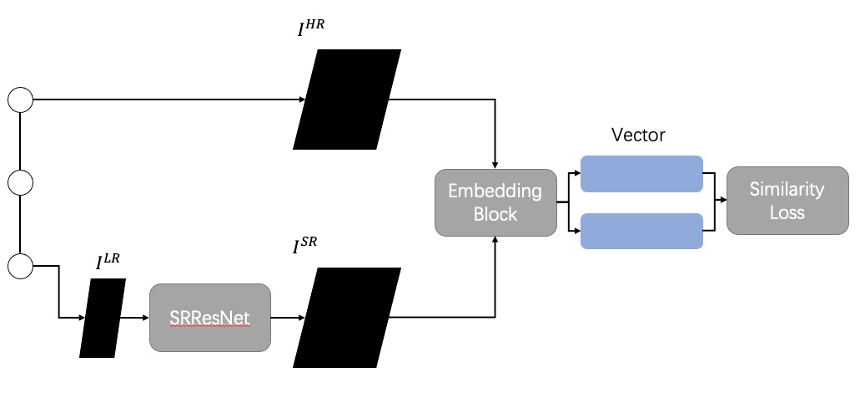
\includegraphics[width=0.86\linewidth]{TrjSR.png}
  \caption{基于TrjSR深度学习模型的时间序列相似性度量}
  \label{fig:TrjSR}
\end{figure}

\section{时间序列模式挖掘}
正如引言所述,随着信息技术的普及和发展,各行各业,尤其是工业领域,
通过相应的传感器和信息系统积累了大量的时间序列数据,
对特定领域或者特定模式的时间序列数据,利用数学建模、
机器学习等方法,进行建模和分析,从而得到特定类型的时间序列子模式,
是一项非常有价值的研究课题。本节将针对诸多业内研究者针对时间序列
模式挖掘问题提出的多种计算和优化方法进行详述。

\subsection{基于相似性检索的模式挖掘方法}
文本领域中,相似性检索方法在包括社区发现、重复检测、聚类和查询细化都有应用\cite{DBLP:conf/www/BayardoMS07}。
Eamonn Keogh将相似性检索算法扩展到了时间序列领域,通过计算时间序列子序列的全对相似性,识别蕴含在时间序列中的所有模式
\cite{DBLP:conf/kdd/RakthanmanonCMBWZZK12}。该算法使用滑动窗口截取了时间序列的全部子序列,使用归一化的欧几里得距离度量两个时间子序列的距离。为了能加速计算,提升算法的时间效率,该算法被设计成了迭代算法,每次随机抽取一个时间子序列,计算其和全部其他时间子序列的欧几里得距离,从而更新距离最小的时间子序列对的信息。为了利用所有时间子序列中大量的重叠信息,该算法使用离散傅里叶变换算法对原始时间序列进行逆变换,进而计算选中子序列和完整时间序列的距离。该方法具有较强的可扩展性,对于超大规模的数据集,
可以随时计算近似结果
\cite{DBLP:conf/icdm/ZhuZSYFMBK16}。

基于相似性检索的模式挖掘方法在对称模式挖掘上具有较大的局限,该方法只能计算出任意两对时间子序列的相似度,却无法判断其是否属于对称子序列。如需挖掘对称模式,当在Matrix Profile算法计算过程中加入子序列对称性的判断,降低算法的时间效率。而且,Matrix Profile算法使用欧氏距离度量两个时间子序列的相似性,由第5章的实验可知,欧几里得距离度量时间序列的相似性忽略了子序列的位置信息从而导致识别不准,在精确率上不如本文设计的对称模式挖掘算法。

\subsection{基于时间序列分解的模式挖掘方法}
在时间序列分析和预测领域,时间序列分解是十分常用的一种方法,
STL(Seasonal-Trend decomposition procedure based on Loess)\cite{DBLP:conf/www/BayardoMS07}
时间序列分解方法基于LOESS\cite{DBLP:books/lib/HastieTF09}
将某时刻的数据分解为趋势分量,周期分量和余项这三个分量,从而挖掘时间序列中蕴含的周期信息和趋势信息。相比于经典的时间序列分解算法,STL并不依赖于移动平均模型,它允许对过程的属性进行分析,对于大量的趋势和季节性的平滑,也可以进行快速计算,并且可以灵活地调整季节性的周期,而不会被数据中的异常行为扭曲。

然而,基于时间序列分解的模式挖掘方法,仅可用于挖掘对称模式为季节模式的时间序列,不能挖掘任意类型的对称模式。真实工业场景中的时间序列数据类型复杂,变化较多,对称模式并不一定呈季节性出现,更可能存在季节性对称模式和非季节性对称模式随机出现的情况。对于该类型的时间序列数据,使用STL算法进行计算往往就不能充分地挖掘出所有的对称模式,或者挖掘出错误的对称模式。

\section{本章小结}
本章定义了论文研究对象的一些相关概念,包括时间序列,
对称子序列和对称模式。由于时间序列对称性的度量本质上
就是计算时间序列两段子序列的对称性,
因此,本章对时间序列相似性度量方法的国内外研究
进行了分类介绍,
主要包括两种类型,
即基于序列形状的相似性度量方法和
基于数学模型的相似性度量方法。
其中基于数学模型的方法不仅增加了复杂性,
在实际度量效果中也不如基于序列形状的方法,
其优点只在于可以通过低维向量进行快速检索。
因而,本文借鉴基于序列形状的方法设计了时间序列对称性度量方法。
由于目前没有成熟的对称模式挖掘算法,
本文随后调研了时间序列一般模式挖掘的相关研究。
结合模式挖掘和距离度量算法,
本文将在后面章节介绍如何在时间序列数据上挖掘对称模式。